\subsection{Parameter and Computation Tradeoffs}
\begin{figure}[t]
\centering
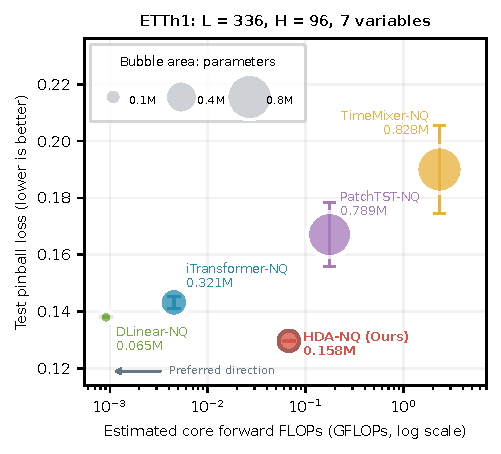
\includegraphics[width=\columnwidth]{figures/efficiency_bubbles.pdf}
\caption{Parameter--accuracy tradeoff on ETTh1 at $H=96$.}
\Description{A bubble plot compares five models by estimated forward FLOPs, test pinball loss, and trainable parameter count. HDA-NQ has the lowest mean pinball and the second-smallest parameter count.}
\label{fig:complexity}
\end{figure}
Figure~\ref{fig:complexity} compares forecasting accuracy, model size, and estimated computation on ETTh1 at $L=336$ and $H=96$. Bubble area denotes trainable parameters, and pinball is the three-seed mean with sample-standard-deviation error bars. Computation is estimated for one full seven-variable input window. HDA-NQ uses 157,960 trainable parameters, compared with 788,732 for PatchTST-NQ, 828,233 for TimeMixer-NQ, and 320,750 for iTransformer-NQ. DLinear-NQ is smaller at 64,718 parameters. Thus, the observed accuracy does not require the largest parameter budget, although the architectures have different tuning histories.

HDA-NQ requires approximately 0.0672 GFLOPs per forward pass under this accounting, with a multiply--add counted as two operations. DLinear-NQ and iTransformer-NQ require less computation, while PatchTST-NQ and TimeMixer-NQ require more. The estimates include sampled attention and key/value interpolation in HDA-NQ, but exclude normalization, nonlinear activations, softmax, miscellaneous elementwise operations, and memory indexing or copying. They support a parameter--accuracy comparison in this setting, not a training-speed or memory-efficiency claim.
